\documentclass{article}

\usepackage[utf8]{inputenc}
\usepackage{geometry}
\usepackage{graphicx}

\usepackage{algorithm}% http://ctan.org/pkg/algorithms
\usepackage{algpseudocode}% http://ctan.org/pkg/algorithmicx

\usepackage{hyperref}
\usepackage{amsmath}


\usepackage{float}

\delimitershortfall-1sp
\newcommand\abs[1]{\left|#1\right|}


\title{Algoritmo: Buscar el par de puntos mas cercano en espacio n-dimensional}
\author{Sergio García Prado}


\begin{document}

\begin{titlepage}
	\centering
	{\scshape\LARGE Universidad de Valladolid \par}
	\vspace{1cm}
	{\scshape\Large Programación Dinámica\par}
	\vspace{1.5cm}
	{\huge\bfseries Subsecuencia Común Más Larga\par}
	\vspace{2cm}
	{\Large\itshape Sergio García Prado\par}
	
	\vfill
	Seguimiento del trabajo en: \par
	\href{https://github.com/garciparedes/Longest-Common-Subsequence}{https://github.com/garciparedes/Longest-Common-Subsequence}

	\vfill


% Bottom of the page
	{\large \today\par}
\end{titlepage}

\section{Introducción}
	
	\subsection{Definición del problema}
	
		\paragraph{}
		El problema analizado que se pretende resolver consiste en lo siguiente:
		
		\paragraph{}
		Primeramente describiremos lo que es una secuencia para despues explicar qué es una subsecuencia, ya que es una de las ideas fundamentales que habrá que tener claro para resolver el problema y que no debemos confundir con subcadena.
		
		\paragraph{Secuencia:}
		Es una colección ordenada de elementos en la cual la repetición está permitida.

		\paragraph{Subsecuencia:}
		Es una secuencia que se obtiene a partir de otra secuencia de igual o mayor tamaño mediante la supresión de algunos elementos sin cambiar el orden de los elementos restantes. Por ejemplo, la secuencia A, D, F es una subsecuencia de A, B, C, D, E, F. 
		\newline
		No debe confundirse con el término subcadena, que además impone la restricción de que los elementos tienen que ser contiguos. Un ejemplo de subcadena es B, C, D.
		
		\paragraph{}
		Ahora que ya tenemos clara la definición de subsecuencia modelizaremos el problema a resolver:
		\newline
		Dadas dos secuencias de carácteres, nuestro objetivo será encontrar la subsecuencia común de mayor longitud entre ambas. La longitud cada una de las cadenas puede ser distinta.

	\subsection{Aplicaciones}
		\paragraph{}
		Este algoritmo tiene una gran cantidad de aplicaciones. Uno de los sectores donde su uso está más extendido es en el de la informática: se usa en software de control de versiones como \textbf{git} o el comando \textbf{diff} de linux, que muestra las diferencias entre ficheros. También se utiliza en el sector de la bioinformática (Aplicación de tecnología de computadores a la gestión y análisis de datos biológicos.) para \textbf{secuenciación de ADN}.

\section{Programación Dinámica}
	\subsection{Definición}
		\paragraph{}
		La programación dinámica es un patrón de diseño de algoritmos basado en la división del problema base que se pretende resolver, en subproblemas de menor tamaño y complejidad que solo se resolverán una única vez, ya que se almacenará la solución de cada uno de ellos para luego reutilizarlo en el caso de que fuera necesario. Al proceso de almacenar las soluciones de los subproblemas se le conoce con el nombre de "memoization". Para que un problema pueda ser resuelto mediante programación dinámica este tiene que cumplir dos propiedades: Solapamiento de Problemas y Subestructura Óptima.

	\subsection{Solapamiento de Problemas}
		\paragraph{}
		Se dice que un problema tiene esta propiedad si este se puede subdividir en problemas de menor tamaño cuyos resultados se pueden reutilizar para resolver sucesivos subproblemas. El ejemplo más claro de esta propiedad es la Sucesión de Fibonacci que se define como:
	
		\[
   		 F(n)= 
			\begin{cases}
    				n,				& \text{if } n\leq 1\\
    				F(n-1)+F(n-2),		& \text{otherwise}
			\end{cases}
		\]
		
		\paragraph{}
		Gráficamente esto se puede representar como un arbol binario, en el cual como vemos para calcular un nodo, tenemos que recurrir a los resultados de sus dos hijos, y así sucesivamente hasta llegar a F(0) o F(1):
		
		\begin{figure}[H]
				\centering
				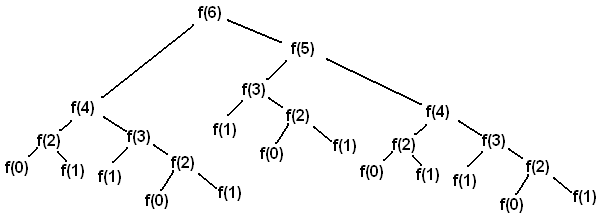
\includegraphics[width=120mm]{../res/fibonacci-sequence.png}
				\caption{Sucesión de Fibonacci \label{example_border}}
		\end{figure}

	\subsection{Subestructura Optima}
		\paragraph{}
		La segunda propiedad que debe cumplir el problema es la de subestructura óptima, que consiste en encontrar la solución optima del problema a partir de soluciones óptimas de sus subproblemas.

\section{Solución}
	\subsection{Enfoques Disponibles}

	\subsection{Programación Dinámica}

	\subsection{PseudoCódigo}

\section{Referencia Bibliográfica}

	\begin{itemize}
		\item \url{https://en.wikipedia.org/wiki/Sequence}	
		\item \url{https://en.wikipedia.org/wiki/Subsequence}	
		\item \url{https://en.wikipedia.org/wiki/Bioinformatics}	
		\item \url{https://en.wikipedia.org/wiki/Dynamic_programming}	
		\item \url{https://www.cs.berkeley.edu/~vazirani/algorithms/chap6.pdf}	
		\item \url{https://en.wikibooks.org/wiki/Algorithms/Dynamic_Programming}	
		
		
		
	\end{itemize}

\end{document}
